\documentclass[pdftex,12pt,letter]{article}
\usepackage[margin=0.75in]{geometry}
\usepackage{verbatim}
\usepackage{graphicx}
\usepackage[pdftex,pdfpagelabels,bookmarks,hyperindex,hyperfigures]{hyperref}

\newcommand{\fixme}[1]{\textbf{#1}}

\setcounter{tocdepth}{1}

\title{BNL Physics Department Intensity Frontier\\Computing Requirements for FY2017-2022}
\date{\today}

\begin{document}
\maketitle
\tableofcontents

%\input{meta}

\newpage
\section{Overview}
This report presents estimates of the computing needs of
the BNL Physics Department Intensity Frontier (IF) efforts for FY2017-2022.
Each of the following sections provides  information for one
experiment or R\&D effort in the BNL Intensity Frontier.
In addition to general information, each section contains a g per-year breakdown of activity and
milestones and resource estimates.

\subsection{Current Status}

The Intensity Frontier (IF) activities at BNL include the following
experiments and research and development efforts:
%
Daya Bay,
LAr1-ND/SBN,
DUNE,
MicroBooNE,
Muon g-2,
Prospect and
WbLS R\&D.
%
Each of these projects are detailed in the following sections but some
commonalities are worth noting here.

Many of the individuals working on these projects participate in more
than one.
This can be done efficiently in part because there are many
overlapping aspects.
For example, MicroBooNE and DUNE  use the same detector
simulation and reconstruction framework, and many of the same
framework modules for their liquid argon detectors.
Software and computing use cases cover a range of scenarios
from individual one-off R\&D software projects to bona fide production
processing and large scale data movement and storage.
One has to look for ways to accommodate this spectrum in an efficient
manner.  

The main computing resource  we rely on to do this is the RHIC/ATLAS Computing
Facility (RACF). Because the RACF is extremely efficient and embodies substantial computing
expertise they have been able to provide Daya
Bay and DUNE a modest footprint at a low direct cost to the experiments.
The footprint of the Daya Bay and DUNE computing at RACF is illustrated in Table \ref{tab:bnlif_at_racf_2016}.
Historically, to the extent that the IF computing does not add to the overall complexity of RACF it
was accommodated with minor incremental effort.


\begin{table}[tbh]
\centering
\begin{tabular}[h]{|l|r|r|r|r|}
  \hline
  Exp. & Purchases & Nodes (boxes) & CPU (cores) & Disk (TB) \\
  \hline
  Daya Bay & 3 & 12 & 296 & 100 \\
  \hline
  DUNE & 1 & 10 & 160 & 55 \\
  \hline
\end{tabular}
\caption{The current (2016) BNL Intensity Frontier Research footprint in RACF.}
\label{tab:bnlif_at_racf_2016}

\end{table}

\subsection{General Strategy}

The BNL IF group intends to continue to leverage RACF. In terms of managing accounts and resources,
we find that the current model of equating an experiment with an RACF Unix account group does not
scale well in our case. Some groups are quite small. There is also to a substantial overlap in group membership
and functions performed by the personnel working in the IF research area.
Without generalization, we note that in this particular case having an experiment-specific,
fine-grained account management setup is cumbersome and complicates the RACF support unnecessarily,
given the significant commonality in the work being done and the tools utilized in the IF research.

The other issue has to do with balancing the immediate and modest needs of
the smaller BNL IF experiments with the costs, minimal as they are, which are
inherent in ``buying into'' the RACF. For example, if an experiment only needs a fraction of a node now (i.e. a few cores),
it is more cost efficient if they can share part of an existing computer and to hold
off purchases until their needs reach the level of at least full node.
Same can be argued about storage and other computing needs.
This has knock-on benefits that waiting always leads to more computing
power for the same cost.

It appears optimal to form an IF umbrella group which will serve to consolidate future RACF hardware purchases
and resource allocations and will then share them among all BNL IF efforts. This will require some additional
self-management by the IF members and group leaders but will reduce overall complexity. The RACF personnel
will need to deal with a single entity instead of a few, thus simplifying support and systems configuration.

%Consolidation can be achieved by directing all new RACF-related purchases by
%the BNL IF members through the new IF umbrella group.

Another activity of such umbrella group is reconfiguration of existing (older) computers,
such as those which belong to the Daya Bay and DUNE clusters. However, potential benefits of doing
this are somewhat decreased by the fact that most of these servers are past their nominal
end-of-life and the effort that needs to be invested into such reconfiguration.

\subsection{Caveats and Clarifications}

\subsubsection{Timeline}
The timeline considered in this document covers FY2017 through FY2022 (nominally 5 years), however where needed
the FY2016 activities are also listed to reflect important work being finalized at the time of writing.
A few of the projects/experiments are scheduled to end before FY2022, which is reflected in the material presented.

\subsubsection{Interpretation of Tables}

In the following sections, tables of hardware
requirements are presented.
The ``Tot.'' column contains the total number of units that are
estimated to be required per year.
For CPU cores this we attempt to estimate the total number of CPU
core-years per year.
Within any given year the usage profile is expected to have peaks
which we must either spread out on our own CPUs or rely on
opportunistic use of the rest of RACF.
As such, this strategy leads to a comfortable overestimate. 
The ``\%New'' columns indicate what portion of that years hardware
unit is expected to be newly purchased that year on the assumption of
the current ``Tot.'' value and given a four year end-of-life for any
hardware from prior years.
We use the ``\%Lab" columns to indicate any computing hardware,
purchased through BNL, but not intended specifically to be used by the
BNL IF efforts. In all cases, we expect no such hardware.

\subsubsection{Hardware End of Life}

The numbers given for RACF hardware assume the nominal four year
end-of-life.
As discussed above, in reality, some longer service life may be
realized.


\subsubsection{Network Bandwidth}
For most of the BNL IF effort, the network requirements can be expected to be quite modest with one
significant exception: DUNE protoDUNE (see Section\,\ref{sec:dune}).


%%%%%%%%%%%%%%%%%%%%%%%%%%%%%%%%%%%%%%%%%%%%%%%%%%%%%%%%%%%%%%%%
\pagebreak
\section{DUNE}
\label{sec:dune}
\subsection{The Far Detector and its prototypes}
The Deep Underground Neutrino Experiment (DUNE) has a variety of important goals that
include:
determination and detailed measurement of CP violation in the neutrino sector,
neutrino mass hierarchy, search for proton decay and observation of neutrinos from supernovae.
It will combine a powerful wide-bandwidth neutrino beam, a fine-grained Near Detector and
the Far Detector based on a uniquely large Liquid Argon TPC (40kt fiducial mass). For the latter,
there are two technologies being actively studied in DUNE: single-phase and dual-phase Liquid Argon TPCs.
In order to validate both designs, an ambitious prototype program (``protoDUNE'') has been initiated which calls
for construction and test-beam operation of two detectors at CERN in late 2018. Before the LHC Long Shutdown.
There is a high probability that a second run will take place during the next LHC run, so protoDUNE is indeed a long
term and large scale project.

The  prototypes are called ``full-scale''
since both will incorporate principal structural elements (such as sensor electrode planes) built according to the scale
of the full DUNE detector. Earlier in 2016, a smaller 35t LArTPC prototype took cosmic ray data at FNAL.

The protoDUNE program is a challenging endeavor which will involve a large cryogenic detector,
state-of-the-art readout technology and signal processing, modern DAQ and other online systems and will require sophisticated calibrations
and processing of a few PB of data. For this reason, in the next few years DUNE software and computing
can be roughly described as two closely related
categories -- DUNE and protoDUNE -- as described below:
\begin{enumerate}

\item DUNE
\begin{itemize}
\item General DUNE ``physics tools'' effort which includes the beam and target studies, the Near Detector
simulation and reconstruction, and simulation and reconstruction with large-scale LAr TPCs of the Far Detector.

\item DUNE DAQ and other online computing R\&D.

\item General computing infrastructure for long-term use during the commissioning and operation of the experiment.
\end{itemize}

\item protoDUNE
\begin{itemize}
\item Near term infrastructure work such as design of protoDUNE DAQ and the online buffer
\item Data transfer and management systems
\item Calibration software, reconstruction algorithms and other application development to support the protoDUNE program.
\end{itemize}
\end{enumerate}

\subsection{Raw Data Handling in protoDUNE}
BNL IF personnel is closely involved in the design of the raw data handling system for protoDUNE.
A conceptual diagram of the system us presented in Fig.\,\ref{fig:raw_concept}. Similar to the
LHC experiments, protoDUNE will leverage EOS as the central element for managing and distributing
the raw data, including to tape storage at CERN and FNAL. Likewise, a specialized online buffer (similar
in function to the ATLAS SFO) will be required to handle substantial data rate that protoDUNE will create
according to the run plan. Plans exist to leverage the Fermi FTS system for implementation of the data
transfer from the online buffer to EOS, and also from EOS to remote data centers (e.g. FNAL, BNL, etc).

BNL IF is currently working on the design of the online buffer. A few technologies are being considered
according to the required performance and ease of integration. The XRootD storage clustering is currently
a very likely technology selection. Initial testing is under way, and integration testing for the online buffer
and Fermi FTS are being planned. Doing this at BNL will require a modest amount
of hardware and basic support.


\begin{figure}[tbh]
\centering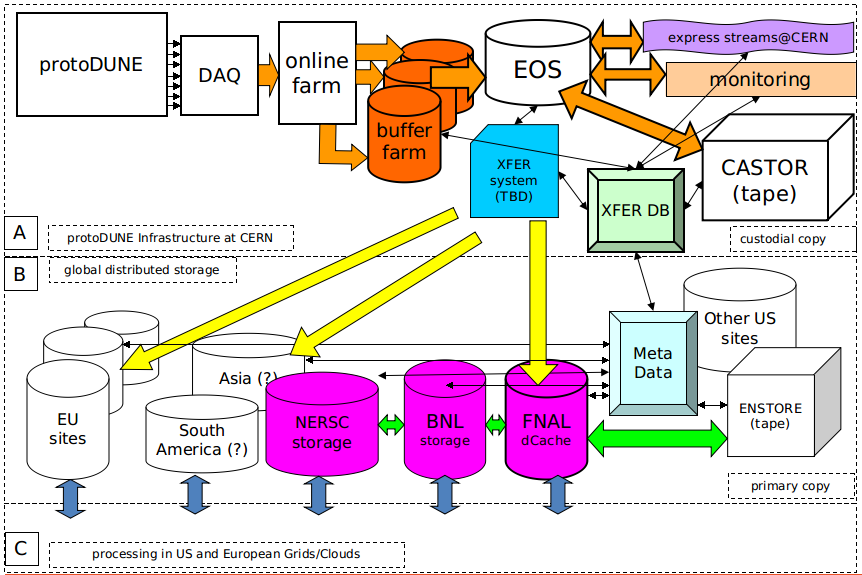
\includegraphics[width=0.8\linewidth]{protoDUNE_raw_data_concept.png}
\caption{\label{fig:raw_concept}Conceptual diagram of the flow of raw data in protoDUNE}
\end{figure}

\subsection{DUNE Offline Computing at BNL}
According to the DUNE Computing Model and the TDR under development at the time of writing,
DUNE will implement a fully distributed data management system. Similar to other experiments,
data (including the raw data) will be replicated to several locations. In addition to managed
replicas existing at major computing sites, we expect that data to be  served to DUNE
researchers and facilities through modern, high-bandwidth, low
latency methods based on combination of XRootD and dCache. Small scale initial testing
of such system took place in 2015, whereby the data residing in dCache at FNAL were read
at BNL via XRootD.

A useful outcome of implementing this system for use in DUNE will be to leverage
investment in BNL's RACF, and to
provide continuity of expertise necessary for the eventual
full-experiment data taking, which according to some plans may take
place around 2024, with a large portion of the Far Detector
commissioned and taking initial data before the arrival of the beam.

In the area of physics tools, BNL plays an important role in the development of software for the detector R\&D (e.g. complex
calculations of electrostatic field in 3D with realistic detector geometry), reconstruction software for DUNE, and
in particular a novel tomography-based approach for LArTPC reconstruction, called ``Wirecell''.


\subsection{protoDUNE Computing Challenges}
While there are still a few unknowns in the run plan and data characteristics of protoDUNE, certain
reliable ``ballpark'' estimates have been created. Currently the nominal number of events to be recorded by the single-phase
protoDUNE detector is fixed at 25\,M, and the total amount of raw data is of the order of 3\,PB. It has been recongized
that this scale (which is an order of magnitude larger than initial estimates) does not fit into ad-hoc single-site processing paradigm
and requires leveraging a few computing sites in addition to FNAL. This creates unique opportunities for BNL as well as substantial challenges.

For BNL RACF to make a meaningful contribution of protoDUNE production and to justify the cost and effort, we estimate that at
the very least 20\% of data would need to be fully processed at BNL within a year of the end of run. Based on this, the storage requirement is 2\,PB of tape and
a commensurate amount of disk space (about 1\,PB) to ensure efficient production.

The required CPU budget is extremely difficult to calculate since all algorithms considered for reconstruction in DUNE (and there are
a few) are under active development, undergo substantial evolution every few months and realistically are quite far from any
sort of meaningful optimization. Still, based on recent experience, it is not unreasonable assume a 5 minutes per track ballpark estimate.
%(the required time will obviously depend on the track length which can be anything from millimeters to meters, so an average is assumed here).
Since most of the occupancy in the TPC will be due to cosmic ray events it is not crucial to conisder the beam event characteristics in
great detail. Given the nominal 5\,ms readout window and estimated values for the cosmic muon flux it is expected that about 50
tracks (and/or track fragments) wil need to be reconstructed in each event. This corresponds to $\sim$4 CPU$\times$hr per reconstructed
event. In keeping with the assumption of 20\% of total statistics to be processed, this resuls in the total CPU budget of 20\,M CPU
hours total for a production run, over the period of about a year. Reprocessing and other additional processing will take place
at a later time but will of course require continued use of the computing resource.

A somewhat unrelated but practically important issue is that of the choice of the Workload Management System for protoDUNE
(and for DUNE beyond that).
A decision is to be made by the DUNE S\&C leadership after consultation with the collaborators and facilities. No such decision has
been made yet at the time of writing.

\subsection{Network Implications}
At the time of writing, no decision has been made on whether the protoDUNE data will be replicated to BNL directly from CERN
EOS  or it iss committed to mass storage at FNAL first and then replicated to BNL. Assuming that the goal is to create a copy of
the raw data sample at about same rate as it is produced by the protoDUNE DAQ, the minimal required network bandwidth (incoming into
BNL) is 300MB/s. This may be revised upward but likely not more than a factor of 2 at the most.

\subsection{Activities and Milestones}
\begin{description}
\item[FY2016] \
\begin{itemize}
\item Analysis of the data taken with the 35t Liquid Argon prototype at FNAL
\item Characterization and improvement of reconstruction algorithms, including Wirecell proof of principle and initial characterization
\item Simulation and reconstriction development for the Near Neutrino Detector
\item Initial preparations for the protoDUNE experiment at CERN (R\&D for DAQ and the online buffer, plans for detector characterization, reconstruction algorithms and framework)
\item Workload Management System technology downselect
\end{itemize}
\item[FY2017] \
\begin{itemize}
\item protoDUNE: prototyping of the online buffer and its DAQ interface, functional and scalability testing
\item protoDUNE: prototyping of the data management system, which will transport the data from the experiment to mass storage at CERN and FNAL, as well as other sites which potentially include BNL
\item protoDUNE: integration of the beam instrumentation systems and data
\item protoDUNE: data challenges involving a few distributed sites
\item protoDUNE: prototype of XRootD data storage federation
\item DUNE: advanced MC studies for rare and background-sensitive physics
\item DUNE: improved Wircell reconstruction framework
\end{itemize}

\item[FY2018] \
\begin{itemize}
\item Installation of the protoDUNE detector at CERN, deployment and integration of the computing and software infrastructure for protoDUNE
\item Readiness of the protoDUNE production and analysis software
\item Commissioning and operation of protoDUNE at CERN
\item Initial analysis of the protoDUNE data
\end{itemize}

\item[FY2019] \
\begin{itemize}
\item Reprocessing of the protoDUNE data
\item Tune-up of reconstruction algorithms using the protoDUNE data
\item DUNE: Initial Far Detector Technology downselect
\item DUNE: Commencement of the Far Detector Stage 1 construction
\item DUNE: Initial Front-End and Online Systems development
\end{itemize}

\item[FY2020-FY2022] \
\begin{itemize}
\item Continued detailed analysis of the protDUNE data
\item Development and deployement of infrastructure for the data distribution and analysis for the 2024-- DUNE commissioning run
\item Deployment and testing of DAQ/Online systems
\item Data challenges for MC and reconstruction
\end{itemize}
\end{description}

\noindent Numbers presented in the following section are based on our
estimates of hardware investments necessary for BNL to meaningfully
support these activities and milestones. 
Our approach is to create a modest but functional pool of CPU power,
and skew the planned hardware capability to storage, in order to meet
relevant items of the software and computing requirements as mentioned
above.  We assume no end-of-life for tapes.

\subsection{Hardware}

\begin{tabular}[h]{|r || r|r|r || r|r|r || r|r|r || r|r|r ||}
  \hline
   & \multicolumn{3}{c||}{Nominal CPU (cores)} & \multicolumn{3}{c||}{Special CPU} & \multicolumn{3}{c||}{Disk (TB)} & \multicolumn{3}{c||}{Tape (TB)} \\
   \hline
  FY & Tot. & \%New & \%Lab & Tot. & \%New & \%Lab & Tot. & \%New & \%Lab & Tot. & \%New & \%Lab \\
  \hline
  2016  &  320 &  100   & 0 & - & - & - & 500 & 100 & 0 & 1000 & 100 &  0 \\
  \hline
  2017 &  320 &   0     & 0 & - & - & - & 500  & 0 & 0 & 1000 & 0    &  0 \\
  \hline
  2018 &  2,300 &   90     & 0 & - & - & - & 1000  & 50   & 0 & 2000 & 50      &  0 \\
  \hline
  2019  &  2,300 &  0    & 0 & - & - & - & 1000  &  0 & 0 & 2000 & 0     &  0 \\
  \hline
  2020 &  2,300 &  0     & 0 & - & - & - & 2000  & 75   & 0 & 2000 & 0    &  0 \\
  \hline
\end{tabular}

%%%%%%%%%%%%%%%%%%%%%%%%%%%%%%%%%%%%%%%%%%%%%%%%%%%%%%%%%%%%%%%%
\pagebreak
\section{Daya Bay}

The Daya Bay reactor antineutrino ($\bar\nu_e$) experiment has been
operating in southern China since December 2011 and expects to
complete operations at the end of FY2017. There are approximately 220
collaborators mainly from China and the US. The yearly US contribution
to Daya Bay operations is approximately \$450k.
Daya Bay makes precision measurements of $\bar\nu_e$ oscillations as
well as the flux and spectrum of reactor antineutrinos. 
Additional measurements include cosmogenic production of neutrons and
isotopes and the cosmic ray muon flux. 
BNL has contributed to the oscillation, flux and spectral measurements
and plans to do so in the future. The current effort is focussed on
reducing the uncertainty in the estimate of the absolute $\bar\nu_e$
detection efficiency from $\sim\!2\%$ to $1\%$ or less. This
uncertainty dominates the uncertainty in the reactor flux measurement. 

The main computing resource in Daya Bay is PDSF at LBNL. BNL provides
a node for automated building and testing of the Daya Bay software
that uses approximately 1 CPU-core-hour each day and 200 GB of disk.
In addition, the existing RACF hardware has been used for simulation
studies as well as some data analysis, and 
it is expected that existing nodes and opportunistic use can provide
the needed hardware and so no new purchase is expected.


\subsection{Activities and Milestones}

\begin{description}
\item[FY2016] Publication of precision reactor flux analysis result. 
				Refinement of oscillation analysis methodology. 
\item[FY2017] Completion of operations. Completion of oscillation analysis methodology. 
\item[FY2018] Publication of final oscillation analysis results.
\item[FY2019] Publication of final reactor flux and spectrum analysis results.
\item[FY2020] Final Daya Bay publications.
\end{description}

\subsection{Hardware}

\begin{tabular}[h]{|r || r|r|r || r|r|r || r|r|r || r|r|r ||}
  \hline
   & \multicolumn{3}{c||}{Nominal CPU (cores)} & \multicolumn{3}{c||}{Special CPU} & \multicolumn{3}{c||}{Disk (TB)} & \multicolumn{3}{c||}{Tape (TB)} \\
   \hline
  FY & Tot. & \%New & \%Lab & Tot. & \%New & \%Lab & Tot. & \%New & \%Lab & Tot. & \%New & \%Lab \\
  \hline
  2017 & 150& 0& 0& -& -& -& 100& 0 & 0 & -& -& - \\
  \hline
  2018 & 100& 0& 0& -& -& -& 50& 0 & 0 & -& -& - \\
  \hline
  2019 & 50& 0& 0& -& -& -& 50& 0 & 0 & -& -& - \\
  \hline
 2020 & 50& 0& 0& -& -& -& 50& 0& 0& -& -& - \\
  \hline
\end{tabular}


%%%%%%%%%%%%%%%%%%%%%%%%%%%%%%%%%%%%%%%%%%%%%%%%%%%%%%%%%%%%%%%%
\pagebreak
\section{LAr1-ND/SBN}

% name, physics goals, collaborators and size, international, approximate cost, stages through the 5 years.

% largely ripped from the CDR

The Fermilab Short Baseline Neutrino program includes the construction
of a Liquid Argon Near Detector, LAr1-ND, at 110 m from the Booster
neutrino source in a new enclosure.
It will serve as the near detector in a a few LAr-TPC experiments
capable of definitively addressing existing anomalies in neutrino
physics and making precision measurements of high-$\Delta m^2$
neutrino oscillations through both appearance and disappearance
searches.
Due to the high event rate of neutrino interactions at the near
location, significant physics output can be achieved with a relatively
short run of the LAr1-ND experiment.  

The collaboration consists of about 100 collaborators from 20
international institutions.
It is expected to cost \$30M US-equivalent and begin operations in
2018. 

The computing requirements to support LAr1-ND are somewhat coupled to
those of MicroBooNE due to their timescales, similarities in
technology and the individuals working on the two efforts at BNL.
It is expected that as MicroBooNE finishes taking data the hardware
dedicated to it will transition to supporting LAr1-ND.
In the table below we do not count this MicroBooNE hardware.

\subsection{Activities and Milestones}

\begin{description}
\item[FY2018] Initial commissioning and data taking with beam begins.
\item[FY2019-2022] Analysis and publications
\end{description}

\subsection{Hardware}

\begin{tabular}[h]{|r || r|r|r || r|r|r || r|r|r || r|r|r ||}
  \hline
   & \multicolumn{3}{c||}{Nominal CPU (cores)} & \multicolumn{3}{c||}{Special CPU} & \multicolumn{3}{c||}{Disk (TB)} & \multicolumn{3}{c||}{Tape (TB)} \\
   \hline
  FY & Tot. & \%New & \%Lab & Tot. & \%New & \%Lab & Tot. & \%New & \%Lab & Tot. & \%New & \%Lab \\
  \hline
  2017 &0 &0 &0 &   -& -& -& 0& 0& 0&- &- &- \\
  \hline
  2018 &50 & 100 &0& -& -& -&  50 & 100 & 0 &- &- &-  \\
  \hline
  2019 &100 & 50& 0& -& -& -& 100 & 50 & 0 &- &- &-  \\
  \hline
  2020 &150 & 33& 0& -& -& -& 150 & 33 & 0 &- &- &-  \\
  \hline
  2021 &150 & 0& 0& -& -& -& 150 & 0 & 0 &- &- &-  \\
  \hline
  2022 &150 & 0& 0& -& -& -& 150 & 0 & 0 &- &- &-  \\
  \hline
\end{tabular}



\pagebreak
\section{MicroBooNE}

The goals of the MicroBooNE experiment include investigating the nature of 
MiniBooNE low energy excess, measuring neutrino-argon interacting cross section,
and R\&D for liquid argon time projection chamber (LArTPC) detector technology 
and reconstruction techniques. It includes over 160 collaborators from 
25 institutions and is led by FNAL. The total cost of the experiment is about 
\$20M. The main detector is a ~80 ton fiducial volume LArTPC located in the 
FNAL Booster neutrino beam line. 

MicroBooNE just finished its CD4, and will start the data taking in March 2015. 
The bulk computing needs of MicroBooNE will be supplied by FNAL and 
thus we do not go into detail here. The BNL computing is expected to supply
the needs of BNL physicist in analyzing MicroBooNE data. The BNL MicroBooNE
physics analysis team contains three staff scientists and five post-docs. 

As noted above, it is expected that MicroBooNE hardware usage will
transition to supporting LAr1-ND.
Only expected purchases initially meant for MicroBooNE are counted in
this section.


\subsection{Activities and Milestones}

\begin{description}
\item[FY2016] Data taking, improve the LArTPC simulation and reconstruction software, data analysis towards publications.
\item[FY2017] Finish data taking and begin work on the cross section publications.
\item[FY2018-2019] Analysis and publications.
%\item[FY2018] 
%\item[FY2019] 
%\item[FY2020]
\end{description}

\subsection{Hardware}

\begin{tabular}[h]{|r || r|r|r || r|r|r || r|r|r || r|r|r ||}
  \hline
   & \multicolumn{3}{c||}{Nominal CPU (cores)} & \multicolumn{3}{c||}{Special CPU} & \multicolumn{3}{c||}{Disk (TB)} & \multicolumn{3}{c||}{Tape (TB)} \\
   \hline
  FY & Tot. & \%New & \%Lab & Tot. & \%New & \%Lab & Tot. & \%New & \%Lab & Tot. & \%New & \%Lab \\
  \hline
  2016 &100 &100 &  0  &- & - & - &50 &100 & 0 &- & - & - \\
  \hline
  2017 &200 &50  &  0  &- & - & - &100 &50 & 0 &- & - & - \\
  \hline
  2018 &200 &0   &  0  &- & - & - &100 & 0 & 0 &- & - & - \\
  \hline
  2019 &100 &0   &  0  &- & - & - & 50 & 0 & 0 &- & - & - \\
  \hline
  2020 &0   &0   &  0  &- & - & - &  0 & 0 & 0 &- & - & - \\
  \hline
\end{tabular}

\pagebreak
\section{Muon g-2}

The goal of the Muon $g-2$ Experiment E989 at Fermilab is to measure
the muon anomalous magnetic moment, $a_\mu \equiv (g-2)/2$, to
unprecedented precision of 0.14~parts per million (ppm).
In the relevant 5 year period the Project will be progressing though
the CD-3, CD-4, commissioning, physics data taking and data analysis.  

The measurement involves ambitious statistical and systematic
uncertainty goals. 
To meet the statistical goal of E989, about $2\times 10^{11}$ events
of muon decay are needed in the final fitted histogram. 
This translates into about two petabytes of data storage requirement
to save the raw experimental data for the offline analysis. 
To meet the systematics goal of E989, both dedicated measurements and
detailed Monte Carlo simulations are needed. 
The simulations require both CPU power and storage capacity,
and are based on the tools recognized by
the HEP community such as {\tt Geant4}, {\tt ROOT}, {\tt MARS}, {\tt
  G4beamline}, {\tt MAD}, {\tt BMAD}. 
%The {\tt Art} framework was chosen by the collaboration as a universal
%data analysis and simulation framework.
%It allows to integrate different software tools into one system, it
%standardizes the event exchange between data producers and data
%consumers, it hides the complexity of low-level data input/output
%protocols, it provides a convenient way to vary the geometry of the
%apparatus as well as the running conditions, it provides a flexible
%mechanism of setting up sophisticated event selection conditions and
%it helps to reduce coding errors by encouraging the users to follow
%the principles recommended by the modern high-level programming
%languages.

\subsection{Activities and Milestones}

\begin{description}
\item[FY2016] 
Generate a $10^9$ muon sample in the storage ring (done mostly at FNAL)
\item[FY2017] 
  Generate a high-statistics data sample using complete end-to-end simulations. 
  Analysis of systematic effects using the generated data sample. 
  Beam tuneup. 
\item[FY2018] 
  Physics data production starts at full beam intensity. 
  BNL resources will be used to store a second copy of experimental data for redundancy and offline data analysis. 
  We expect to collect a comparable to or twice as high statistics of muon decays of the previous Muon $g-2$ experiment E821 at Brookhaven. 
  Analysis of experimental data starts. 
\item[FY2019] 
  Continue physics data production. 
  Collect $5\div 10\times$ the statistics of the BNL experiment. 
  Analysis of experimental data.  
  First physics result. 
\item[FY2020]
  The full statistics collected. Data analysis.  
\end{description}

\noindent Following the strategy of the previous Muon $g-2$ experiment at Brookhaven, the collaboration is
planning to establish two or more parallel efforts of data analysis and evaluation of systematic uncertainties by
independent groups of people and independent analysis algorithms.  Computing resources at BNL will be used for
the independent analysis of the experimental data and to study the systematic effects. 
The data storage requirements in the table below include the storage for both simulated and physics data. 

\subsection{Hardware}

\begin{tabular}[h]{|r || r|r|r || r|r|r || r|r|r || r|r|r ||}
  \hline
   & \multicolumn{3}{c||}{Nominal CPU (cores)} & \multicolumn{3}{c||}{Special CPU} & \multicolumn{3}{c||}{Disk (TB)} & \multicolumn{3}{c||}{Tape (TB)} \\
   \hline
  FY & Tot. & \%New & \%Lab & Tot. & \%New & \%Lab & Tot. & \%New & \%Lab & Tot. & \%New & \%Lab \\
  \hline
  2016 & 150 & 100 &  0& - &- &- & 10 & 100 & 0& 100 &  100 & 0\\
  \hline
  2017 & 300 &  50  & 0& - &- &- &  50 &  80    &0 & 500 &   90 & 0\\
  \hline
  2018 & 300 &   0   & 0& - &- &- &  50 & 0      &0 & 1000 &   80 & 0\\
  \hline
  2019 & 300 &   0   & 0& - &- &- & 100 & 50     &0 & 3000 &   60 & 0\\
  \hline
  2020 & 300 &  50  &  0&-  &- &- & 100 &  10    &0 & 6000 &   50 & 0\\
  \hline
\end{tabular}

%%%%%%%%%%%%%%%%%%%%%%%%%%%%%%%%%%%%%%%%%%%%%%%
\pagebreak
\section{PROSPECT}

The PROSPECT reactor antineutrino experiment's goals are to understand
reactor antineutrino emissions and resolve the "reactor anomaly". The
PROSPECT collaboration is largely based in the US with approximately
50 collaborators and is expected to grow to $\sim\!65$. 
The experiment will measure $\bar\nu_e$ inverse beta decay interactions
with segmented, ${}^6{\rm Li}$-loaded liquid scintillator (LiLS)
detectors.

The main computing resources for PROSPECT are expected to be LLNL and
Yale University. The BNL effort is on design and simulation of the passive shielding,
simulation of calibration using short-lived radioactive isotopes
dissolved in the liquid scintillator and analysis of detector
data. The initial computing effort would leverage the Daya Bay RACF
hardware. 
\subsection{Activities and Milestones}

\begin{description}
\item[FY2016] Construction and deployment of the Phase I 2-ton near detector at HFIR.
				Analysis of Phase I detector data. R\&D towards a Phase II far detector.
\item[FY2017] Near detector operation. Planning for far detector (if desired based on near
			detector results).
\item[FY2018] Near detector operation. 
\item[FY2019] Construction and deployment of far detector, if warranted.
\item[FY2020] Near and far detector operation, if warranted.
\end{description}

\subsection{Hardware}

\begin{tabular}[h]{|r || r|r|r || r|r|r || r|r|r || r|r|r ||}
  \hline
   & \multicolumn{3}{c||}{Nominal CPU (cores)} & \multicolumn{3}{c||}{Special CPU} & \multicolumn{3}{c||}{Disk (TB)} & \multicolumn{3}{c||}{Tape (TB)} \\
   \hline
  FY & Tot. & \%New & \%Lab & Tot. & \%New & \%Lab & Tot. & \%New & \%Lab & Tot. & \%New & \%Lab \\
  \hline
  2016 & 50 &100 &0 &- &- &- & 10& 100&0 &- &- &- \\
  \hline
  2017 & 100& 50& 0&- &- &- & 20& 50&0 &- &- &-  \\
  \hline
  2018 & 100& 0& 0&- &- &- & 20& 0&0 &- &- &-  \\
  \hline
  2019 & 100& 0& 0&- &- &- & 20& 0&0 &- &- &-  \\
  \hline
  2020 & 100& 50& 0&- &- &- & 20& 50&0 &- &- &-  \\
  \hline
\end{tabular}

%%%%%%%%%%%%%%%%%%%%%%%%%%%%%%%%%%%%%%%%%%%%%%%%%%%
\pagebreak
\section{Water-based Liquid Scintillator R\&D}
New techniques developed by the BNL electronic detector and neutrino
\& nuclear chemistry group for Water-based Liquid Scintillator (WbLS)
formulation allow the fraction of scintillating liquid in water to be
varied. 
The personnel of the R\&D effort are two BNL scientists, a staff
member, a full-time postdoc and occasional contributions from others
in the electronic detector and neutrino \& nuclear chemistry groups.   
The goals of the R\&D effort are to measure the properties of WbLS
with sufficient detail to be able to predict the light yield for
ionizing particles in large-scale detectors.

The main computing effort is the analysis of prototype data and the development of a detailed
simulation model. In addition, plans exist and work is under way to implement and commission a 
$\sim$\,1000 liter WbLS detector.

Computation work is done collaborators' laptops and RACF. A small, but sustained, hardware
presence in RACF is foreseen going forward.

\subsection{Activities and Milestones}

\begin{description}

\item[FY2016-18] Operation of $\sim$\,1000 liter WbLS detector. Data analysis.
                \item [FY2019-20] Characterization of WbLS. 
\end{description}

\subsection{Hardware}

\begin{tabular}[h]{|r || r|r|r || r|r|r || r|r|r || r|r|r ||}
  \hline
   & \multicolumn{3}{c||}{Nominal CPU (cores)} & \multicolumn{3}{c||}{Special CPU} & \multicolumn{3}{c||}{Disk (TB)} & \multicolumn{3}{c||}{Tape (TB)} \\
   \hline
  FY & Tot. & \%New & \%Lab & Tot. & \%New & \%Lab & Tot. & \%New & \%Lab & Tot. & \%New & \%Lab \\
  \hline
  2016 & 10 & 100& 0&- &- &- & 2& 100 & 0&- &- &- \\
  \hline
  2017 & 10&    0& 0&- &- &- & 2& 0& 0&- &- &-  \\
  \hline
  2018 & 10&    0& 0&- &- &- & 2& 0& 0&- &- &-  \\
  \hline
  2019 & 10&    0& 0&- &- &- & 2& 0& 0&- &- &-  \\
  \hline
  2020 & 10&  100& 0&- &- &- & 2& 100& 0&- &- &-  \\
  \hline
\end{tabular}




\end{document}
